\graphicspath{{images/}}

\section{\thesection~Introduction}
\label{sec:introduction}

% Expand motivation, describe QFA, discuss alternative approaches.

Dummy \citet{Lawless2010} citations \citep{Heydari2016} \citep{Addinall2008}.

\subsection{\thesubsection~Subsection}

\begin{Figure}
  \centering
  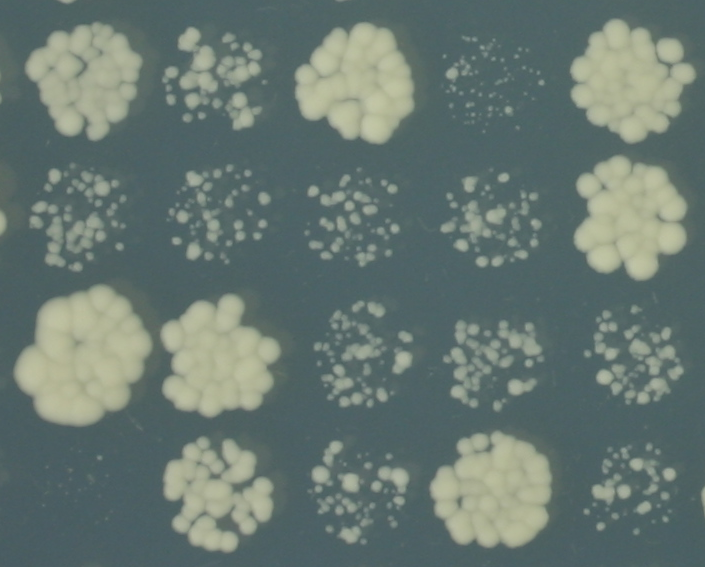
\includegraphics[width=\linewidth]{p15_section/p15_section}
  \captionof{figure}{\textbf{4x5 section of a QFA plate.} Taken from a
    16x24 format solid agar plate inoculated with dilute
    \textit{S. cerevisae} cultures.
  Image captured at \(\sim\)2.5d after inoculation and incubation at
  27\(^{\circ}C\).}
  \label{fig:p15_section}
\end{Figure}


\begin{Figure}
  \centering
  \includegraphics[width=\linewidth]{stripes/final/striped}
  \includegraphics[width=\linewidth]{stripes/final/filled}
  \captionof{figure}{\textbf{An experiment designed to examine
      competition.}\\
    A) QFA plate inocluated with a more concentrated
    \textit{S. Cerevisae} inoculum (no cells inocluated on alternative
    columns).\\
    B) Same as in A, but with strains of similar growth rate
    inoculated in the positions missing in A.}
  \label{fig:stripes_images}
\end{Figure}



%%% Local Variables:
%%% mode: latex
%%% TeX-master: "report"
%%% End:
